\documentclass{article}
\usepackage[ruled,vlined]{algorithm2e}
\usepackage{amsfonts}
\usepackage{amsmath}
\usepackage{amssymb}
\usepackage{amsthm}
\usepackage[UKenglish]{babel}
\usepackage{bm}
\usepackage{booktabs}
\usepackage[capitalise]{cleveref}
\usepackage{dashbox}
\usepackage{fullpage}
\usepackage[utf8]{inputenc}
\usepackage[UKenglish]{isodate}
\usepackage{mathtools}
\usepackage{tikz}
\usepackage{xcolor}
\usepackage{xfrac}
\usepackage[backgroundcolor=lightgray]{todonotes}
\usepackage{soul}
\usepackage{mathrsfs}
\usepackage{capt-of}
\usepackage{siunitx}

\newtheorem{theorem}{Theorem}
\newtheorem{proposition}{Proposition}
\newtheorem{lemma}{Lemma}
\newtheorem{corollary}{Corollary}
\newtheorem{conjecture}{Conjecture}
\theoremstyle{definition}
\newtheorem{definition}{Definition}
\newtheorem{example}{Example}
\theoremstyle{remark}
\newtheorem*{remark}{Remark}

\title{Weighted Model Counting Without Parameter Variables}

\begin{document}

\maketitle

% TODO: make introduce an acronym: project-join tree = PJT
\section{Main Results}

\paragraph{Notation.} For any propositional formula $\phi$ and $p, q \in
\mathbb{R}_{\ge 0}$,
\[
  [\phi]^p_q \coloneqq
  \begin{cases}
    p & \text{if } \phi \\
    q & \text{otherwise.}
  \end{cases}
\]

\todo[inline]{Formal definition of a previous WMC instance (CNF, literal weight
  function) and the new definition (set of $2^{X} \to \mathbb{R}_{\ge 0}$
  pseudo-Boolean functions and a constant). Note that the constant idea is
  borrowed from \texttt{bklm16}.}

\paragraph{References.}
\begin{itemize}
\item `Apply' is quadratic \cite{DBLP:journals/tc/Bryant86}.
\item Related work without publicly available implementations:
  \begin{itemize}
  \item direct compilation to SDDs \cite{DBLP:conf/ecsqaru/ChoiKD13}
  \item direct compilation to PSDDs, also eliminating parameter variables (a thesis)
  \item maybe two more papers
  \end{itemize}
\end{itemize}
% TODO: do a literature search focused around these papers

\paragraph{Notes.}
\begin{itemize}
\item Let $X_P$ be the set of parameter variable and $X_I$ be the set of
  indicator variables.
\item Parameter variables are either taken from the LMAP file (for encodings
  produced by Ace) or assumed to be the variables that have both weights equal
  to 1.
\item If a parameter variable in a clause is `negated', we can ignore the
  clause. We assume that there are no clauses with more than one instance of
  parameter variables.
\item The second \textbf{foreach} loop can be performed in constant time by
  representing $\phi'$ as a list and assuming that the two 'clauses' are
  adjacent in that list (and incorporating it into the first loop).
\item The $d$ map is constructed in $\mathcal{O}(|X_P|\log|X_P|)$ time (we want
  to use a data structure based on binary search trees rather than hashing).
\item \texttt{rename} can be implemented in $\mathcal{O}(\log |X_P|)$ time.
\item Apparently, the DPMC paper already shows that taking the first offered
  decomposition tree is best.
\item This may look like preprocessing, but all the transformations are local
  and thus can be incorporated into an encoding algorithm with no slowdown. In
  fact, if anything, the resulting algorithm would be slightly faster, as it
  would have less data to output.
\item It is already well-known that WMC is FPT.
\end{itemize}

\begin{algorithm}
  \caption{WMC instance transformation}
  \SetKwFunction{rename}{rename}
  \SetKwProg{Fn}{Function}{:}{}
  \KwData{an (old-format) WMC instance $(\phi, X_I, X_P, W)$}
  \KwResult{a (new-format) WMC instance $(\phi', \omega)$}
  $\phi' \gets \emptyset$\;
  $\omega \gets 1$\;
  let $d\colon X_P \to \mathbb{N}$ be defined as $v \mapsto |\{ u \in X_P \mid u
  \le v \}|$\;
  \ForEach{clause $c \in \phi$}{
    \uIf{$c \cap X_P = \{ v \}$ for some $v$ \textnormal{\textbf{and}} $W(v) \ne
      1$}{
      \uIf{$|c| = 1$}{$\omega \gets \omega \times W(v)$\;}
      \Else{
        $\phi' \gets \phi' \cup \left\{ \left[ \bigwedge_{l \in c \setminus
              \{v\}} \neg l \right]^{W(v)}_1 \right\}$\;
      }
    }
    \ElseIf{$\{v \mid \neg v \in c\} \cap X_P  = \emptyset$}{
      $\phi' \gets \phi' \cup \{ [c]^1_0 \}$\;
    }
  }
  \ForEach{indicator variable $v \in X_I$}{
    \If{$\{[v]_1^p, [\neg v]_1^q\} \subseteq \phi'$ for some $p$ and $q$}{
      $\phi' \gets \phi' \setminus \{ [v]_1^p, [\neg v]_1^q \} \cup \{ [v]_q^p
      \}$\;
    }
  }
  replace every variable $v$ in $\phi'$ with $\rename{$v$}$\;
  \Return{$(\phi', \omega)$}\;
  \Fn{\rename{$v$}}{
    $S \gets \{u \in X_P \mid u \le v\}$\;
    \lIf{$S = \emptyset$}{\Return{$v$}}
    \Return{$v - d(\max S)$}\;
  }
\end{algorithm}

\section{Parameterised Complexity of DPMC}

% NOTE: By DPMC, we always mean DMC+lg.
% TODO: maybe use texttt for DPMC?

Summary:
\begin{itemize}
\item We establish DPMC inference as fixed-parameter tractable.
\item We show that, in the case of cw, the parameter is the same as in the BN lower bound,
\item and, in the case of d02, the DPMC parameter is exponentially higher.
\item We experimentally show that cw+DPMC is best on low-to-moderate treewidth
  instances, and cd06+c2d overtakes cw+DPMC on higher treewidth instances.
\end{itemize}

Define:
\begin{itemize}
\item treewidth of a graph,
\item Boolean formula in CNF (perhaps this is too trivial to define),
\item primal graph of a CNF formula (a.k.a.
  Gaifman/(variable) interaction/connectivity/clique/representing graph),
\item Bayesian network (I already have a definition of these last two),
\item moralisation of a Bayesian network (or of any DAG),
\end{itemize}

\begin{theorem}[\cite{DBLP:conf/ecai/KwisthoutBG10}, rephrased]
  BN Inference (for all algorithms that accept arbitrary instances) has a lower
  bound that's linear in the size of the BN and exponential in the treewidth of
  its moralisation (provide the exact formula).
\end{theorem}

\begin{definition}[\cite{DBLP:conf/cp/DudekPV20}, verbatim]
  Let $X$ be a set of Boolean variables and $\phi$ be a CNF formula over $X$. A
  \emph{project-join tree} (PJT) of $\phi$ is a tuple $(T, r, \gamma, \pi)$
  where:
  \begin{itemize}
  \item $T$ is a tree with root $r \in \mathcal{V}(T)$,
  \item $\gamma\colon \mathcal{L}(T) \to \phi$ is a bijection between the leaves
    of $T$ and the clauses of $\phi$, and
  \item $\pi\colon \mathcal{V}(T) \setminus \mathcal{L}(T) \to 2^X$ is a
    labelling function on internal nodes.
  \end{itemize}
  Moreover, $(T, r, \gamma, \pi)$ must satisfy the following two properties:
  \begin{enumerate}
  \item $\{\pi(n) : n \in \mathcal{V}(T) \setminus \mathcal{L}(T)\}$ is a
    partition of $X$, and
  \item for each internal node $n \in \mathcal{V}(T) \setminus \mathcal{L}(T)$,
    variable $x \in \pi(n)$, and clause $c \in \phi$ such that $x$ appears in
    $c$, the leaf node $\gamma^{-1}(c)$ must be a descendant of $n$ in $T$.
  \end{enumerate}
\end{definition}

\begin{definition}[\cite{DBLP:conf/cp/DudekPV20}]
  \[
    \mathtt{Vars}(n) \coloneqq
    \begin{cases}
      \mathtt{Vars}(\gamma(n)) & \text{if } n \in \mathcal{L}(T) \\
      \left( \bigcup_{o \in \mathcal{C}(n)} \mathtt{Vars}(o) \right) \setminus
      \pi(n) & \text{if } n \not\in \mathcal{L}(T).
    \end{cases}
  \]
  \[
    \mathtt{size}(n) \coloneqq
    \begin{cases}
      |\mathtt{Vars}(n)| & \text{if } n \in \mathcal{L}(T) \\
      |\mathtt{Vars}(n) \cup \pi(n)| & \text{if } n \not\in \mathcal{L}(T).
    \end{cases}
  \]
  The \emph{width} of a PJT $(T, r, \gamma, \pi)$ is
  $\mathtt{width}(T) \coloneqq \max_{n \in \mathcal{V}(T)} \mathtt{size}(n)$.
\end{definition}

\begin{theorem}[\cite{DBLP:conf/cp/DudekPV20}, paraphrased, `ADD width is equal
  to the treewidth of the primal graph']
  Given a CNF formula $\phi$ with a tree decomposition of its primal graph of
  width $w$, Algorithm~2 (from \cite{DBLP:conf/cp/DudekPV20}) returns a
  PJT of $\phi$ of width at most $w+1$.
\end{theorem}

\begin{figure}
  \centering
  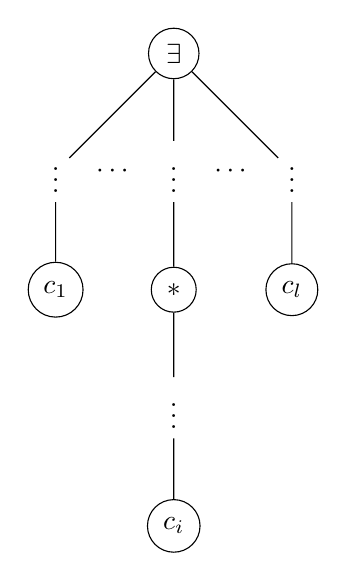
\begin{tikzpicture}
    \node[circle,draw] {$\exists$}
    child {node (a) {$\vdots$}
      child {node[circle,draw] {$c_1$}}
    }
    child {node (b) {$\vdots$}
      child {node[circle,draw] {$\ast$}
        child {node {$\vdots$}
          child {node[circle,draw] {$c_i$}}
        }
      }
    }
    child {node (c) {$\vdots$}
      child {node[circle,draw] {$c_l$}}
    }
    ;
    \path (a) -- (b) node[midway] {$\cdots$};
    \path (b) -- (c) node[midway] {$\cdots$};
  \end{tikzpicture}
  \caption{An example PJT with clauses $c_1, \dots, c_i, \dots, c_l$ that all
    contain the same variable, its projection node $\exists$, and a node under
    consideration $\ast$.}
\end{figure}

\begin{lemma}
  The number of variables that can appear in the ADDs within a PJT node is $\le
  k+1$.
\end{lemma}
\begin{proof}
  All such variables are introduced in a `clause' below and projected either in
  this node or in one of its ancestors. Each such variable would be in the bag
  of each clause that introduced it. By the tree decomposition properties, it
  will also be in the bag of both the projection node and the current node
  because they are on the path between the clause nodes (see the figure).
\end{proof}

\begin{theorem}
  \textsc{DPMC} is FPT w.r.t. the PJT width. More specifically,
  \textsc{DPMC} running time is $\mathcal{O}(4^km(n+k))$, where $k$ is the
  width, $n$ is the number of clauses, and $m$ is the number of variables.
\end{theorem}
\begin{proof} % TODO: finish
  \begin{itemize}
  \item An ADD with $k$ variables can have up to $2^0 + 2^1 + \dots + 2^k =
    2^{k+1} - 1 = \mathcal{O}(2^k)$ nodes (including leaves).
  \item Multiplying $m$ ADDs can then take up to $(m-1)(2^{k+1}-1)^2 =
    \mathcal{O}(m4^k)$ (since one multiplication takes up to $(2^{k+1}-1)^2$
    time and the and the result will have up to $2^{k+1} - 1$ nodes because the
    domain stays the same).
  \item Each projection consists of two linear operations and a quadratic
    operation, so projecting $m$ variables will take $\mathcal{O}(4^km)$ time.
  \item In total, operations on a PJT node with $m$ ADDs, $k$ variables, $n$ of
    which are projected takes $\mathcal{O}(4^k(m+n))$ time.
  \item The total time taken by the DPMC execution stage is the sum of the time
    taken `inside' each PJT node. The number of such nodes is upper bounded by
    $m$, so the total time complexity of DPMC is $\mathcal{O}(4^km(n+k))$.
  \end{itemize}
\end{proof}

\bibliographystyle{acm}
\bibliography{paper}

\end{document}